
\section{Experiments}


\subsection{Part-of-speech tagging}

This section will go into the details of the Part-of-speech task, what the
specifics are, considerations in regards to the data used, any issues we came
across, and the results of our experiments.

\subsubsection{Task definition}

The Part-of-Speech task is a classification task where the objective is to label
each word in a sentence with it's corresponding part-of-speech label such as
noun, verb, adjective, etc. Some languages have more of labels than other. The
same words can have different labels in different context, so the classifier
should be able to figure out the which label is a better fit on a sentence by
sentence basis. Simply remembering that word $X$ has label $Y$ wouldn't be able
to generalize very well.

The performance of a classifier for the POS task is the simple accuracy of the
predictions. Since there are no label which is a lot more common than others
guessing randomly would very rarely give a better accuracy than perhaps 10\%.

\subsubsection{Data}

For this task we used datasets from~\ref{}{UniversalDependencies.org} which has
a broad selection of languages with multiple datasets (called treebanks) in
each. The datasets from~\ref{}{UniversalDependencies.org} are all in the CoNNL-U
format, but are created from different types of sources. The source types are
given as tags such as news, legal, blog, wiki, etc.

Since the datasets from~\ref{}{UniversalDependencies.org} comes pre-split, these
were concatenated before splitting into our own sizes. Concatenation happened
using the command ``cat *.conllu > combined.conllu'', since the convention for
the datasets is to name the files something with train, test, and dev, the
assumed order of the files is dev, test, and train. Meaning that if the dev set
(eg. the validation set) contains 5000 sentence, only these were used in our
datasets, and none of the sentences from the test or training-sets would be
used. No guarantees however were made to guarantee this ordering, so depending
on the naming conventions used in the specific treebanks this might differ.

Some datasets, such as the Norwegian dataset, contains contractions as well as
the individual words. Since the contration is usually unlabelled in the datasets
these were simply removed from the data for ease of parsing. This has the
obvious consequence that the models are not trained on the contractions of words
which are often more commonly used, this however shouldn't affect the
comparisons between word orderings since contractions shouldn't affect these.

The treebanks we selected from~\ref{}{UniversalDependencies.org} were all made
from news, where some used additional sources such as non-fiction and spoken. A
list of the languages, their respective treebank selected, and their tags is
given below.

* Arabic,   PADT, news

* Hindi,    HDTB, news

* Urdu,     UDTB, news

* Japanese, GSD, blog, news

* Danish,   DDT, fiction, news, non-fiction, spoken

* Norwegian,Bokmaal, blog, news, non-fiction

* Russian,  SynTagRus, fiction, news, non-fiction

The distribution of tokens, labels, etc. is given in appendix.

\subsubsection{Results and analysis}


\pagebreak


\subsection{Named Entity Recognition}

This section will go into the details of the Named Entity Recognition task, what
the specifics are, considerations in regards to the data used, any issues we
came across, and the results of our experiments.

\subsubsection{Task definition}

Named Entity Recognition is a classification task of different types of
entities, such as places, people, organisation, times, and more. Entities can
consist of one or more words (and/or numbers), eg.\ ``Eurovision Song Contest
2019'' is a single entity of 3 words and a number. The classifier should
correctly identify the whole entity and not just part of it. We didn't take this
into consideration before running the experiments so our results are on a word
by word basis and doesn't tell us if the whole entity was correctly classified
or not.

The same entity might never show up in the dataset twice so it's important for
the classifier to be able to figure out based on context of the other words in
the sentence if there is an entity or not. It is impossible to simply remember
that a word refers to an entity since the word was most likely not seen during
training.

Usually the performance of a classifier for the NER task is measured by a $F_1$
Score, which considers the classifier's precision and recall. The precision is
the classifier's ability to correctly classify an entity given all attempts, and
recall is the ability to correctly classify an element given how many elements
exists. Say there are 100 entities in a document, the classifier finds 90
entities, 80 of them are correct, 10 of them are wrong, and 20 were not found.
From this we get the precision $P = {80 \over 80 + 10} = 0.88\ldots$, and recall
$R = {80 \over 80 + 20} = 0.8$. The $F_1$ score is simply the harmonic mean
between the precision and recall given by $F_1 = 2 \cdot {precision \cdot recall
\over precision + recall}$. Based on our example this would be $F_1 = 2 \cdot
{0.88 \ldots \cdot 0.8 \over 0.88\ldots + 0.8} = 0.8421$ \cite{f-measure}.

The rationale behind using the $F_1$ score is that usually a lot of the data is
non-entities. A classifier which classified nothing as an entity would have a
great accuracy on datasets with few entities. Since we didn't evaluate if whole
entities were classified correctly, we will base our score on the individual
words and the score might therefore be higher than otherwise. Since we aren't
comparing with models outside our own this shouldn't be an issue.

The reason the NER task is relevant is its usefulness in handling huge data
sizes, since the task is inherently about extracting information from text.
Extracting entities from a text would allow for easy tagging, comparisons
between documents, and linking to a knowledge base. A document mentioning
different locations and capital cities such as ``France'', ``Tokyo'', and ``New
Zealand'', could be about geografi or traveling. And similar a document
mentioning people associated with economy could be about economy
\cite{sang2003introduction}.

The state of the art model for NER based off of \cite{ner-state} is
\cite{baevski2019cloze}. They use a bidirectional self-attention cloze model
which seems very disimilar to anything we are doing. They achieve an F1 score of
93.5 on the CoNLL 2003 English dataset, which is 0.41 points above the previous
state of the art by \cite{akbik2018coling}, the same model mentioned in the
previous section with state of the art results for POS.

\subsubsection{Data}\label{sec:experiments-ner-data}

For the NER task we used auto-annotated wikipedia data from
\cite{pan-etal-2017-cross}. This dataset contains annotated data for 282
languages in varying sizes. 

The datasets are all in the BIO (or IOB) format, which has three different
entities; organisations, people, and locations. The BIO format uses the
convention that the beginning of an entity is prefixes with a B and the
continuation of an entity is prefixed with an I (for inside). Tokens which are
not part of an entity is labeled O (for other). This gives the 7 labels, B-ORG,
B-PER, B-LOC, I-ORG, I-PER, I-LOC, and O. 

Since all the datasets were created based on wikipedia data we didn't have to
take varying sources into considerations, as was necessary for the POS task.

The data being auto-annotated means it might not be of the same standard as the
POS data. Ideally this shouldn't affect the experiments since the word orderings
are still the same, and systematic errors in the data would hopefully happen for
all languages in the datasets.

For Japanese which doesn't use spaces to differentiate between the beginning and
the end of words, the data is split and labeled character by character, this
differs from the POS data where words are split in a more natural way. This has
an influence on the results and means that Japanese isn't as comparable between
tasks as other languages. Since it turns out that our Polyglot embedding has a
somewhat similar way to split words it can have a positive effect on the
performance.

Another issue with the Japanese NER dataset we used is that we ignored many of
the tokens in the dataset by mistake. For the CoNLL-U datasets, the \# symbol is
used for comments. When reading the datasets we simply skipped files starting
with the \# symbol and continued reading normally. This is only an issue for the
Japanese dataset since it was the only one using these symbols, however these
symbols constitudes around 5\% of the data. This is another issue with the
Japanese dataset, and it's hard to say if ignoring these symbols is beneficial
to the experiment or not.

As the data used for training the model is the same data used for training the
polyglot word embeddings, the models don't have the same kind of variety from
the data as is the case for the POS task. This may result in worse performance
since the models might be more likely to overfit.

A table of the languages with the number of entities in their respective dataset
is given below in Table~\ref{table:token-distribution-ner}. 

\begin{table}[h!]
    \centering
    \begin{tabular}{l c c c c c c c c c}
        \toprule
        \multicolumn{10}{l}{\bfseries Training} \\
        Language & Tokens & Distinct &
        B-PER & I-PER & B-LOC & I-LOC & B-ORG & I-ORG & O \\
        
        \cmidrule(lr){1-10}

        ar   &  27159 &  8567 &
        1929 &   3919 &  1835 &  2526 & 1112 &  2237 & 13601 \\

        da   &  35498 & 10247 &
        1419 &   1802 &  3385 &   991 &  974 &  1264 & 25663 \\

        hi   &  23276 &  4667 &
        3502 &   4021 &   700 &   830 & 1105 &  2943 & 10175 \\

        ja   & 122377 &  2429 &
        1644 &   6853 &  1663 &  4420 & 2575 & 10970 & 94252 \\

        no   &  41172 & 10988 &
        1525 &   2076 &  3229 &   943 & 1302 &  1506 & 30591 \\

        ru   &  26232 &  9817 &
        2483 &   5341 &   973 &   711 & 1109 &  2269 & 13346 \\

        ur   &  21391 &  3048 &
         502 &   1549 &   3012 & 10024 & 527 &  1500 &  4177 \\

        \cmidrule(lr){1-10}
        \multicolumn{10}{l}{\bfseries Testing} \\
        Language & Tokens & Distinct &
        B-PER & I-PER & B-LOC & I-LOC & B-ORG & I-ORG & O \\
        
        \cmidrule(lr){1-10}

        ar  & 2991 & 1039 &
         91 &  211 &  230 &  525 &  237 &  652 & 1045 \\

        da  & 4523 & 1682 &
        248 &  352 &  333 &  191 &  138 &  255 & 3006 \\

        hi  & 2884 & 1234 &
        180 &  288 &  110 &  177 &  268 &  892 &  969 \\

        ja  &14723 & 1176 &
        299 & 1730 &  155 &  471 &  229 & 1342 &10497 \\

        no  & 5574 & 1549 &
         25 &   31 &  492 &   65 &  155 &  243 & 4563 \\

        ru  & 2280 &  989 &
        456 & 1095 &   31 &   15 &   33 &   60 &  590 \\

        ur  & 2813 &  310 &
          0 &    0 &  487 & 1745 &   19 &   62 &  500 \\
        \bottomrule
    \end{tabular}
    \caption{Distribution of tokens on the NER data sets for each language.
    }\label{table:token-distribution-ner}
\end{table}

\subsubsection{Model comparison}

Starting by looking at number of epochs trained
(Table~\ref{table:epochs-run-ner}), we see that all models terminated training
some time before hitting the upper bound, with the TensorFlow implementation of
\texttt{Bi-LSTM} with a batch size of 8 being the slowest to converge (36.8
epochs on average). Also, we see that \texttt{Bi-LSTM-CRF} models converged
faster for most every batch size and implementation.

\begin{table}[h!]
    \centering
    \begin{tabular}{l c c c|c c c}
        \toprule
        \multirow{2}{*}{\bfseries Batch size}     &
        \multicolumn{3}{c}{\bfseries Bi-LSTM}     &
        \multicolumn{3}{c}{\bfseries Bi-LSTM-CRF} \\
        \cmidrule(lr){2-7}
        & DyNet & PyTorch & TensorFlow
        & DyNet & PyTorch & TensorFlow \\
        \cmidrule(lr){1-7}
         1 &  9.49 & 13.43 & 21.00 &  8.14 &  7.66 &  6.43 \\
         8 &  9.86 & 22.43 & 36.80 &  9.97 & 11.46 &  8.69 \\
        32 & 12.57 & 29.06 & 31.51 & 11.57 & 14.63 & 10.91 \\
        \bottomrule
    \end{tabular}
    \caption{Average of epochs run across all seeds and languages when trained
        with early stopping.
        }\label{table:epochs-run-ner}
\end{table}

However, when turning our attention to the \textit{F1} scores
(Table~\ref{table:f1-total-ner}), the models are performing very poorly, which
does not fit with the expected results of a well converged model. We suspect the
main reason for this, is the fact that our models did the same \textit{accuracy}
test during training to decide when to stop as was done in the POS task. But
since we for the NER task want to optimize our \textit{F1} score, the accuracy
test is really not the optimal parameter to use in early stopping --- it would
of course had made more sense to test if the \textit{F1} score had stopped
improving.

% F1 SCORE
\begin{table}[h!]
    \centering
    \begin{tabular}{c l c c c|c c c}
        \toprule
        \multirow{2}{*}{\bfseries Language} &
        \multirow{2}{*}{\bfseries Batch size} &
        \multicolumn{3}{c}{\bfseries Bi-LSTM} &
        \multicolumn{3}{c}{\bfseries Bi-LSTM-CRF} \\
        \cmidrule(lr){3-8}
        && DyNet & PyTorch & Tensorflow & DyNet & PyTorch & Tensorflow \\

        \cmidrule(lr){1-8}
        \multirow{3}{*}{\bfseries ar}
        &  1 & 
        \underline{\textbf{83.5}} & 78.6 & 74.3 &
        82.6 & \underline{78.7} & \underline{75.0} \\
        &  8 & 
        \underline{\textbf{82.4}} & 62.5 & 47.4 &
        80.8 & \underline{77.3} & \underline{66.2} \\
        & 32 & 
        79.2 & 42.4 & 27.8 &
        \underline{\textbf{79.3}} & \underline{70.0} & \underline{48.9} \\

        \cmidrule(lr){1-8}
        \multirow{3}{*}{\bfseries da}
        &  1 &
        \underline{\textbf{77.0}} & 70.5 & \underline{54.0} &
        76.9 & \underline{71.8} & 49.9 \\
        &  8 &
        \underline{\textbf{74.9}} & 48.1 & 23.5 &
        74.6 & \underline{69.3} & \underline{35.1} \\
        & 32 &
        68.0 & 27.7 &  0.0 &
        \underline{\textbf{69.2}} & \underline{61.4} & \underline{20.8} \\

        \cmidrule(lr){1-8}
        \multirow{3}{*}{\bfseries hi}
        &  1 &
        \underline{\textbf{69.7}} & \underline{65.3} & 52.2 &
        69.4 & 62.8 & \underline{55.5} \\
        &  8 &
        \underline{\textbf{68.3}} & 55.1 & 26.2 &
        67.3 & \underline{63.4} & \underline{51.2} \\
        & 32 &
        \underline{\textbf{64.0}} & 33.6 &  1.2 &
        62.6 & \underline{56.9} & \underline{37.9} \\

        \cmidrule(lr){1-8}
        \multirow{3}{*}{\bfseries ja}
        &  1 &
        \underline{\textbf{58.1}} & \underline{34.9} & \underline{35.4} &
        52.6 &  8.1 & 14.8 \\
        &  8 &
        \underline{\textbf{54.3}} & \underline{24.9} & 13.6 &
        47.6 & 11.7 & \underline{47.3} \\
        & 32 &
        \underline{\textbf{47.9}} & 22.5 &  9.3 &
        44.5 & \underline{27.8} & \underline{45.2} \\

        \cmidrule(lr){1-8}
        \multirow{3}{*}{\bfseries no}
        &  1 &
        65.2 & \underline{49.7} & 29.9 &
        \underline{\textbf{67.1}} & 44.5 & \underline{47.1} \\
        &  8 &
        \underline{\textbf{63.2}} & 25.4 & \underline{11.8} &
        61.4 & \underline{48.1} &  3.4 \\
        & 32 &
        \underline{\textbf{56.0}} & 18.2 &  \underline{8.3 }&
        50.1 & \underline{37.2} &  2.2 \\

        \cmidrule(lr){1-8}
        \multirow{3}{*}{\bfseries ru}
        &  1 &
        \underline{\textbf{96.6}} & 95.3 & 81.2 &
        96.6 & \underline{95.8} & \underline{93.3} \\
        &  8 &
        96.2 & 93.5 & 68.7 &
        \underline{\textbf{96.4}} & \underline{95.9} & \underline{93.0} \\
        & 32 &
        95.5 & 83.5 & 43.3 &
        \underline{\textbf{95.7}} & \underline{95.2} & \underline{87.2} \\

        \cmidrule(lr){1-8}
        \multirow{3}{*}{\bfseries ur}
        &  1 &
        \underline{97.8} & 96.8 & 95.2 &
        97.4 & \underline{\textbf{98.0}} & \underline{97.6} \\
        &  8 &
        \underline{\textbf{97.8}} & 93.6 & 82.9 &
        97.6 & \underline{97.7} & \underline{96.9} \\
        & 32 &
        96.3 & 84.5 & 71.1 &
        \underline{\textbf{97.4}} & \underline{96.5} & \underline{96.3} \\
        \bottomrule
    \end{tabular}
    \caption{F1 scores for NER experiments by language and batch
        size. Bold: highest accuracy for batch size plus language. Underline:
        highest accuracy for framework between \texttt{Bi-LSTM} and
        \texttt{Bi-LSTM-CRF}.
    }\label{table:f1-total-ner}
\end{table}


Furthermore, the loss function should also have been utilized differently. The
motivation for using the \textit{F1} score, is to focus attention on the models
ability to classify entities and not reward it too much for identifying
`O'-tokens. But for our cross-entropy loss, a true prediction of a tag `O' has
had the same influence as the true prediction of an entity tag. Since there are
a lot more non-entities than entities, it is reasonable to suggest, that the
models will have tuned their parameters to correctly classify non-entities and
accepted a lower accuracy rate for entity tags. This is also supported by the
results shown in Figure~\ref{chart:tag-acc-ner}.

\begin{figure}[h!]
    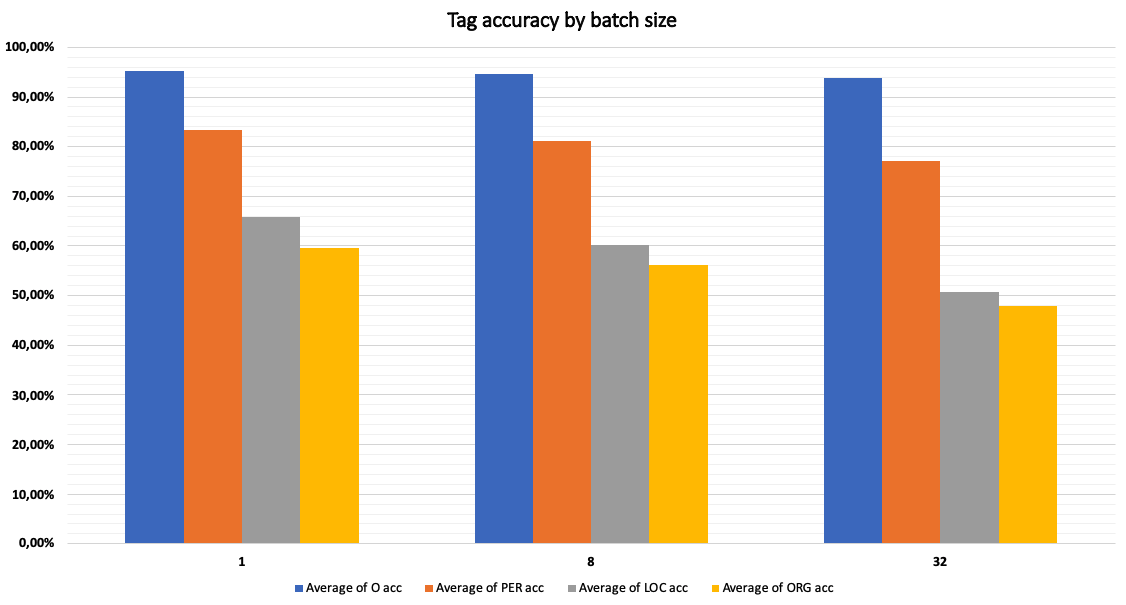
\includegraphics[width=\textwidth]{tag-acc-ner}
    \caption{Column diagram of averaged accuracy percentages for NER tags
        (B-<tag> and I-<tag> are combined in PER, LOC and ORG)
    }\label{chart:tag-acc-ner}
\end{figure}

Despite this design flaw, we still get some notable observations from the
obtained \texttt{F1} scores, depicted in
Figure~\ref{chart:f1-by-batch-and-lang}.  First of all, we once again see that
the DyNet implementations are by far the most succesfull, having the highest
score in all but one experiment. This is again attributed to its 2 layer
implementation of the bidirectional LSTM network. We also see the same pattern
as for POS, where the PyTorch implementation has the second best results and
the TensorFlow implementation is falling severely behind.

We also see, that the \texttt{Bi-LSTM-CRF} models in PyTorch and TensorFlow
outperforms their \texttt{Bi-LSTM} counterparts at almost every batch size and
language (the notable exceptions being cases for Japanese and Norwegian, where
the scores are extraordinarily low. See Section~\ref{sec:experiments-ner-data}
for more). This is interesting, as it confirms the expectation that the CRF
layer is able to significantly improve the performance in performing NER tasks
(~\cite{huang2015bidirectional}).

We still don't see a consistent improvement on the DyNet implementations from
the CRF layer. This again indicate, that the addition of a CRF layer to a 2
layer \texttt{Bi-LSTM} model is of negligible effect for these batch sizes.
However, we might see a small tendency for the larger batch sizes to benefit
from the CRF, as the DyNet \texttt{Bi-LSTM-CRF} model highest score in Arabic,
Danish, Russian and Urdu.

Another observation concerning applying CRF is how much it helps an increasing
batch size. For the pure \texttt{Bi-LSTM} models, a batch size of 32 drops the
performance by 36.4\% for the PyTorch implementation and by a whooping 61.9\%
for the TensorFlow implementation when compared to a batch size of 1. For the
\texttt{Bi-LSTM-CRF} models, these numbers go down to 3.2\% and 20.0\%
respectively. It should be noted, that the \textit{F1} scores for the DyNet
implementation actually experience a slight increase in the perfomance drop from
the larger batch size when CRF is applied (the drop goes from 7.5\% to 8.1\%).

\begin{figure}[h!]
    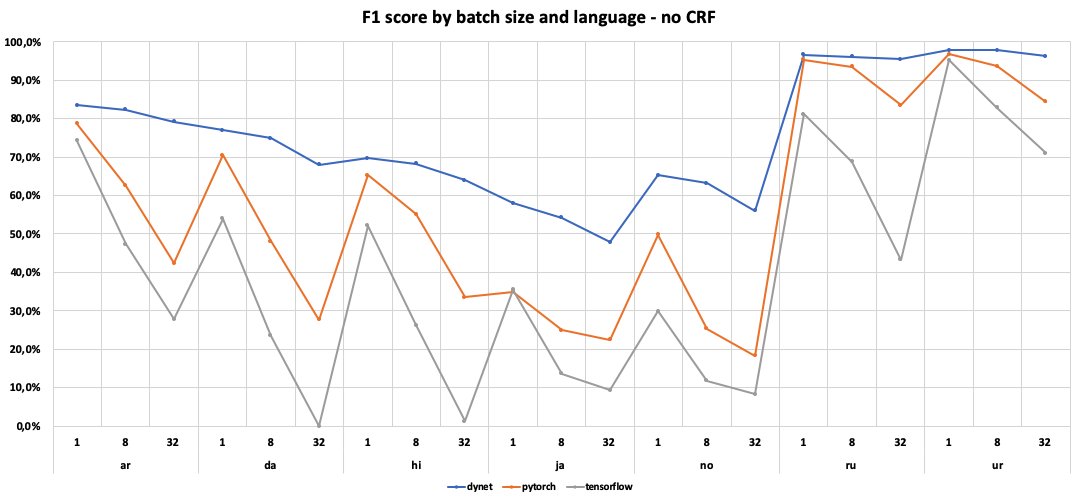
\includegraphics[width=\textwidth]{f1-no-crf}
    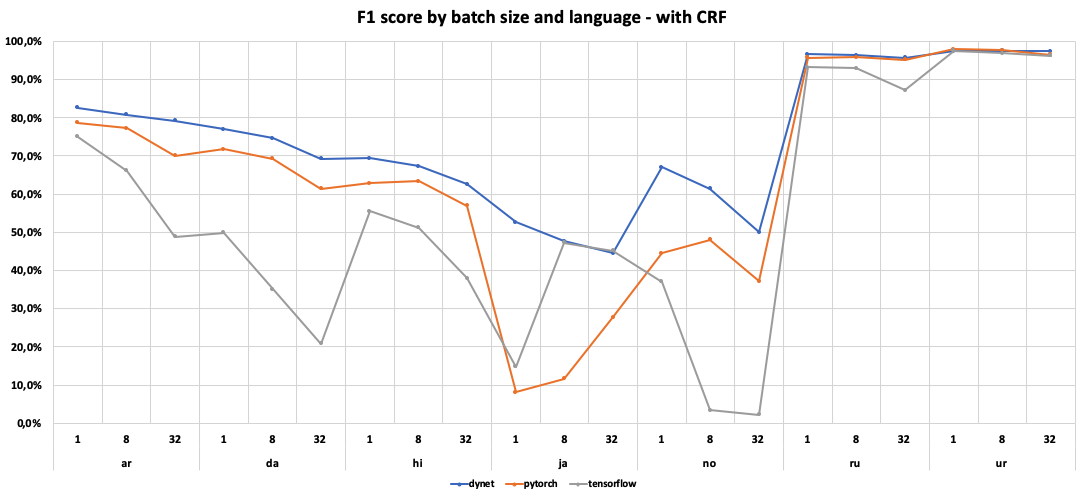
\includegraphics[width=\textwidth]{f1-with-crf}
    \caption{\textit{F1} scores for each framework implementation by batch size
        and language. Notice drops in performance when the batch size increases
        in models that does not utilize a CRF model. Top: the \texttt{Bi-LSTM}
        implementations. Bottom: the \texttt{Bi-LSTM-CRF} implemenations.
    }\label{chart:f1-by-batch-and-lang}
\end{figure}

\subsubsection{Language comparison}\label{sec:experiments-ner-lang-comparison}

Looking at the tag distributions in Table~\ref{table:token-distribution-ner}, we
notice several oddities, that are worth mentioning. As we consider the results,
we therefore first describe some potential problems related to the data, since
we believe they may be the cause of some of the strange values we get. The
results for each language are presented in Table~\ref{table:f1-total-ner} and
plottet in Figure~\ref{chart:f1-by-batch-and-lang}.

The training data for Norwegian looks reasonable when comparing with the other
languages, but for the test data there are very few entities (ie.\ non-`O'
tags). More than 80\% of the tokens are `O' tags which is noticably different
from the other languages. Since the \textit{F1} scores is calculated only on
entities, a large part of the test data is disregarded in this respect, and the
models \textit{F1} score will quickly be punished for misclassifications as each
prediction has a relatively higher weight compared to test data with more
entities.

Arguably the tagger should still be able to identify the entities correctly, no
matter how few there are. However, when looking at the results, we see
significantly lower scores than for most other languages. Adding the CRF layer,
we also observe that the PyTorch and TensorFlow models behave irregularly. For
the PyTorch implementation, the score improves by 3.6 when increasing the
batch size from 1 to 8, but then drops by 10.9 when it is increased to 32. For
TensorFlow, the score for a batch size of 1 is 47.1, but drops to 3.4 and 2.2
for batch size 8 and 32 respectively. In general, the increase in batch size
either leads to a steady decay or improvement of the scores (or only a very
small change one way or the other), so this behaviour is highly irregular.

Japanese has the second highest number of `O' tags which constitute slightly
above 70\% of the total test data. The results are not the same kind of
irregular as for Norwegian, but we do observe an unprecedented and sudden boost
in the perfomance of the TensorFlow \textit{Bi-LSTM-CRF} model over the others.
It especially seems odd, that this implementation --- that in all other cases
gets worse with an increasing batch size --- actually outperforms the
corresponding DyNet implementation at batch size 32. Further, as the only example
of this, the PyTorch \textit{Bi-LSTM-CRF} goes from 8.1 through 11.7 to 27.8 for
increasing batch sizes --- in all other cases, an increasing batch size for
PyTorch leads to decreasing scores. Last but not least, the Japanese scores are
overall by far the worst, so with these irregularities in mind aswell as the
data issues mentioned in Section~\ref{sec:experiments-ner-data}, we assume that
there are flaws in this experiment.

For Russian and Urdu, we observe that the test data almost solely consists of a
single entity type, which believe can make the results very inflated. For the
training data (and not counting `O' tags), Russian had 60.1\% person tags
(either `B-PER' or `I-PER') but for the test data, these tag types made up
91.8\% of the entity tags. For Urdu, the uneven distribution was even more
extreme: during training, 75.7\% of the entity tags were of type `B-LOC' or
`I-LOC' against a massive 96.5\% in the test data.

Add to that, that these two languages both have the lowest number of tokens and
the lowest number of distinct tokens. These facts may have an influence on why
the \textit{F1} scores for Russian and Urdu outperforms every other language.
All three framework implemenations achieve scores of more than 90\%, and the for
a batch size of 1, the PyTorch \texttt{Bi-LSTM-CRF} model reaches a stunning
score of 98.0.

\subsubsection*{Accuracy}

For completeness sake, we also include the data for our results on general
accuracy on the NER data in Table~\ref{table:acc-total-ner}. This was the actual
score our models trained to optimize and are as such relevant. 

Overall they align pretty well with the pattern found in the rest of the data,
but they are expectedly higher. The best results are generally either achieved
by the lowest batch size or by the \texttt{Bi-LSTM-CRF} and always by the DyNet
implementation. The best results reaches pretty impressive heights with
97.3\% for russian and 98.5\% for urdu. However since these accuracy scores can
get pretty high by just being really good at identifying non-entities, the
accuracy may not reflect the practical success of the models.

\begin{table}[h!]
    \centering
    \begin{tabular}{c l c c c|c c c}
        \toprule
        \multirow{2}{*}{\bfseries Language} &
        \multirow{2}{*}{\bfseries Batch size} &
        \multicolumn{3}{c}{\bfseries Bi-LSTM} &
        \multicolumn{3}{c}{\bfseries Bi-LSTM-CRF} \\
        \cmidrule(lr){3-8}
        && DyNet & PyTorch & Tensorflow & DyNet & PyTorch & Tensorflow \\

        \cmidrule(lr){1-8}
        \multirow{3}{*}{\bfseries ar}
        &  1 & 
        \underline{\textbf{88.4}} & \underline{87.4} & \underline{85.4} &
        88.3 & 84.1 & 81.6 \\
        &  8 & 
        \underline{\textbf{88.6}} & \underline{85.5} & \underline{81.1} &
        88.0 & 85.3 & 76.1 \\
        & 32 & 
        \underline{\textbf{88.9}} & 80.9 & \underline{77.0} &
        87.5 & \underline{84.8} & 71.5 \\

        \cmidrule(lr){1-8}
        \multirow{3}{*}{\bfseries da}
        &  1 &
        91.3 & \underline{90.5} & \underline{87.6} &
        \underline{\textbf{91.5}} & 89.8 & 81.6 \\
        &  8 &
        91.2 & 88.0 & \underline{85.3} &
        \underline{\textbf{91.2}} & \underline{90.4} & 75.8 \\
        & 32 &
        \underline{\textbf{91.1}} & 86.2 & 67.1 &
        91.1 & \underline{88.8} & \underline{74.2} \\

        \cmidrule(lr){1-8}
        \multirow{3}{*}{\bfseries hi}
        &  1 &
        \underline{\textbf{75.6}} & \underline{74.0} & \underline{72.0} &
        75.5 & 70.0 & 62.1 \\
        &  8 &
        74.6 & 71.5 & \underline{62.2} &
        \underline{\textbf{74.9}} & \underline{72.9} & 60.7 \\
        & 32 &
        74.3 & 64.8 & 34.4 &
        \underline{\textbf{74.5}} & \underline{70.1} & \underline{53.8} \\

        \cmidrule(lr){1-8}
        \multirow{3}{*}{\bfseries ja}
        &  1 &
        \underline{\textbf{83.7}} & \underline{80.0} & \underline{80.1} &
        81.4 & 52.2 & 72.8 \\
        &  8 &
        \underline{\textbf{82.4}} & \underline{80.5} & 77.8 &
        81.5 & 73.7 & \underline{79.4} \\
        & 32 &
        \underline{\textbf{82.1}} & \underline{79.4} & 77.1 &
        81.3 & 73.8 & \underline{81.0} \\

        \cmidrule(lr){1-8}
        \multirow{3}{*}{\bfseries no}
        &  1 &
        94.4 & \underline{86.4} & 87.2 &
        \underline{\textbf{94.4}} & 74.4 & \underline{87.3} \\
        &  8 &
        95.1 & 77.5 & \underline{85.3} &
        \underline{\textbf{95.3}} & \underline{86.4} & 82.0 \\
        & 32 &
        \underline{\textbf{94.2}} & \underline{85.5} & \underline{84.5} &
        93.1 & 81.7 & 82.1 \\

        \cmidrule(lr){1-8}
        \multirow{3}{*}{\bfseries ru}
        &  1 &
        \underline{\textbf{97.3}} & \underline{96.5} & 90.8 &
        97.1 & 96.1 & \underline{93.6} \\
        &  8 &
        \underline{\textbf{97.2}} & 96.0 & 85.6 &
        97.0 & \underline{97.1} & \underline{93.3} \\
        & 32 &
        96.9 & 94.1 & 72.3 &
        \underline{\textbf{97.1}} & \underline{97.0} & \underline{91.4} \\

        \cmidrule(lr){1-8}
        \multirow{3}{*}{\bfseries ur}
        &  1 &
        \underline{\textbf{98.5}} & 97.8 & 98.1 &
        98.0 & \underline{98.3} & \underline{98.1} \\
        &  8 &
        98.1 & 97.7 & 96.7 &
        \underline{\textbf{98.1}} & \underline{98.4} & \underline{97.2} \\
        & 32 &
        98.2 & 96.1 & 95.4 &
        \underline{\textbf{98.3}} & \underline{97.3} & \underline{96.9} \\
        \bottomrule
    \end{tabular}
    \caption{Accuracy in percentage for NER experiments by language and batch
        size. Bold: highest accuracy for batch size plus language. Underline:
        highest accuracy for framework between \texttt{Bi-LSTM} and
        \texttt{Bi-LSTM-CRF}.
    }\label{table:acc-total-ner}
\end{table}



\pagebreak


\subsection{OOV results}

Comparing the two-layer \texttt{Bi-LSTM-CRF} of DyNet and the one-layer
\texttt{Bi-LSTM-CRF} of PyTorch on their ability to correctly classify
out-of-vocabulary (OOV) words, we see once again that the two-layer model of
DyNet performs slightly better. On average across languages, batch sizes, epochs
and seeds, the two-layer model has an OOV accuracy (ie.\ the percentage of
correctly classified OOV words) of 86.2\% for NER data, where as the one-layer
model only achieves an OOV accuracy 81.0\%. The results are shown in
Table~\ref{table:oov-accuracy-crf}.

\begin{table}[h!]
    \centering
    \begin{tabular}{l c c c c}
     \toprule
     \multirow{2}{*}{\bfseries Epochs}
     & \multicolumn{2}{c}{\bfseries NER}
     & \multicolumn{2}{c}{\bfseries POS} \\
              & DyNet  & PyTorch & DyNet  & PyTorch \\ \cmidrule(lr){1-5}
     1        & 81.8\% & 76.4\%  & 81.8\% & 87.8\%  \\
     5        & 87.5\% & 82.8\%  & 91.3\% & 91.0\%  \\
     patience & 89.3\% & 83.9\%  & 92.8\% & 91.8\%  \\ \cmidrule(lr){1-5}
     \bfseries Total & 86.2\% & 81.0\%  & 88.4\% & 90.2\% \mdseries \\
     \bottomrule
    \end{tabular}
    \caption{OOV accuracy for the \texttt{Bi-LSTM-CRF} models implemented in
        DyNet (two-layer model) and in PyTorch (one-layer model). The rows
        indicate the number of epochs run during training, where `patience'
        refers to a training session with early stopping after 3 consecutive
        epochs of declining accuracy in the validation set.
    }\label{table:oov-accuracy-crf}
\end{table}
 

For POS data, this is not the case, as the average accuracy actually tips in
favour of the one-layer model of PyTorch (88.4\% against 90.2\%). However, when
training using patience to determine when to stop, the upper hand is again with
the two-layer model, which achieves an OOV accuracy of 92.8\% against 91.8\%.
This is a small difference, and it could very well be the result of the PyTorch
implementation, in which it is not the optimal model, that is returned, but the
optimal model after three extra epochs of declining accuracy on the validation
set (see Section~\ref{} for more details).

\pagebreak
